\section{Radionuclide Transport Base Cases}\label{sec:nuclide_base_cases}
\subsection{Basic Transport and Containment Problem Specification}
Basic transport and containment base cases were conducted to verify basic 
transport and contaminant behavior of all the radionuclide transport models at 
each component interface. These tests neglected thermal transport and capacity 
estimation to simplify the verification procedure.  

The problem design includes : 
\begin{itemize}
\item{A source facility providing one waste stream per timestep}
\item{A legislated repository capacity of 5 1kg waste streams}
\item{A waste form Component} 
\item{A waste package Component}
\item{A buffer Component}
\item{A far field Component}
\end{itemize}

\subsubsection{Degradation Rate Model}
The Degradation Rate model should not release contaminants if the degradation 
rate is 0. If the degradation rate is nonzero, however, contaminants should 
become available immediately to the adjacent components, traveling quickly 
accross the interfaces. 

To observe these behaviors, four simulations were run to demonstrate that total 
containment resulted from a degradation rate of 0 and that conrguent release 
resulted from nonzero degradation rates. A description of these verification 
cases can be found in Table \ref{tab:dr_base}. The 0 degradation rate component was 
different for each of the four cases. This resulted in total containment at the 
Waste Form, Waste Package, Buffer, and Far Field interfaces respectively. 
Results of these base cases can be found in Figures 
\ref{fig:drIwf5} through \ref{fig:drIVff0}.

\begin{table}[htp!]
\centering
\footnotesize{
\begin{tabularx}{\textwidth}{|X|X|X|X|X|}
  \multicolumn{5}{c}{\textbf{Degradation Rate Model No Release Contaminant Transport}}\\
  \hline
  \textbf{Case}  &  \textbf{Component} &  \textbf{Degradation Rate} & \textbf{Expected Release 100 yrs} & \textbf{Actual Release 100 yrs}\\
  \textbf{ID}    & \textbf{[Type]} &  \textbf{$[yr^{-1}]$}  &  $[\%]$  & $[\%]$\\
  \hline
  DRI     &  WF    &  0   & 100 & 100\\
          &  WP    &  0.1 & 0 & 0 \\
          &  BUFF  &  0.1 & 0 & 0 \\
          &  FF    &  0.1 & 0 & 0\\
  \hline
  DRII    &  WF    &  0.1 & 0 & 0\\
          &  WP    &  0   & 100 & 100\\
          &  BUFF  &  0.1 & 0 & 0\\
          &  FF    &  0.1 & 0 & 0\\
  \hline
  DRIII   &  WF    &  0.1 & 0 & 0\\
          &  WP    &  0.1 & 0 & 0\\
          &  BUFF  &  0   & 100 & 100\\
          &  FF    &  0.1 & 0 & 0\\
  \hline
  DRIV    &  WF    &  0.1 & 0 & 0\\
          &  WP    &  0.1 & 0 & 0\\
          &  BUFF  &  0.1 & 0 & 0\\
          &  FF    &  0   & 100 & 100\\
  \hline
\end{tabularx}
\caption[Degradation rate model no release problem results.]{Results from demonstration cases for non-release from 0-degradation Degradation Rate modeled Components.}
\label{tab:dr_base}
}
\end{table}


\begin{figure}[ht]
\centering
\includegraphics[width=0.6\textwidth]{./chapters/demonstration/base/drI.eps}
\caption[$^{235}U$ residence. Degradation Rate Waste Form No Release.]{
For Case DRI, in which total containment in the waste form is assumed ($F_{d,wf}=0$), 
$^{235}U$ takes up permanent residence in the waste form component.
}
\label{fig:drIall}
\begin{minipage}[b]{0.45\linewidth}

  \includegraphics[width=\textwidth]{./chapters/demonstration/base/drI1.eps}
  \caption[Case DRI Waste Form Contaminants.]{
    Waste Form 5 ($F_d = 0$) never releases material.
    }
  \label{fig:drIwf5}
  
  \includegraphics[width=\textwidth]{./chapters/demonstration/base/drI3.eps}
  \caption[Case DRI Buffer Contaminants]{
    The Buffer, component 7 ($F_d = 0.1$), never recieves material.
    }
  \label{fig:drIbuff}

\end{minipage}
\hspace{0.05\linewidth}
\begin{minipage}[b]{0.45\linewidth}
  \includegraphics[width=\textwidth]{./chapters/demonstration/base/drI2.eps}
  \caption[Case DRI Waste Package Contaminants.]{ 
    Waste Package 6 ($F_d = 0.1$), never recieves material.
    }
  \label{fig:drIwp6}

  \includegraphics[width=\textwidth]{./chapters/demonstration/base/drI0.eps}
  \caption[Case DRI Far Field Contaminants.]{ 
    The Far Field, component 0 ($F_d = 0.1$), never recieves material.
    }
  \label{fig:drIff0}

  \end{minipage}
\end{figure}
\FloatBarrier



\begin{figure}[ht]
\centering
\includegraphics[width=0.6\textwidth]{./chapters/demonstration/base/drII.eps}
\caption[$^{235}U$ residence. Degradation Rate Waste Package No Release.]{
For Case DRII, in which total containment in the waste package is assumed ($F_{d,wp}=0$), 
$^{235}U$ travels through waste forms ($F_d = 0.1$) before 
permanent residence in the waste package components.
}
\label{fig:drIIall}
\begin{minipage}[b]{0.45\linewidth}

  \includegraphics[width=\textwidth]{./chapters/demonstration/base/drII1.eps}
  \caption[Case DRII Waste Form Contaminants.]{
    Waste Form 5 ($F_d = 0.1$) releases material with degradation. 
    }
  \label{fig:drIIwf5}
  
  \includegraphics[width=\textwidth]{./chapters/demonstration/base/drII3.eps}
  \caption[Case DRII Buffer Contaminants]{
    The Buffer, component 7 ($F_d = 0.1$), never recieves material.
    }
  \label{fig:drIIbuff}

\end{minipage}
\hspace{0.05\linewidth}
\begin{minipage}[b]{0.45\linewidth}
  \includegraphics[width=\textwidth]{./chapters/demonstration/base/drII2.eps}
  \caption[Case DRII Waste Package Contaminants.]{ 
    Waste Package 6 ($F_d = 0$) acheives total containment.
    }
  \label{fig:drIIwp6}

  \includegraphics[width=\textwidth]{./chapters/demonstration/base/drII0.eps}
  \caption[Case DRII Far Field Contaminants.]{ 
    The Far Field, component 0 ($F_d = 0.1$), never recieves material.
    }
  \label{fig:drIIff0}


  \end{minipage}
\end{figure}
\FloatBarrier

\begin{figure}[ht]
\centering
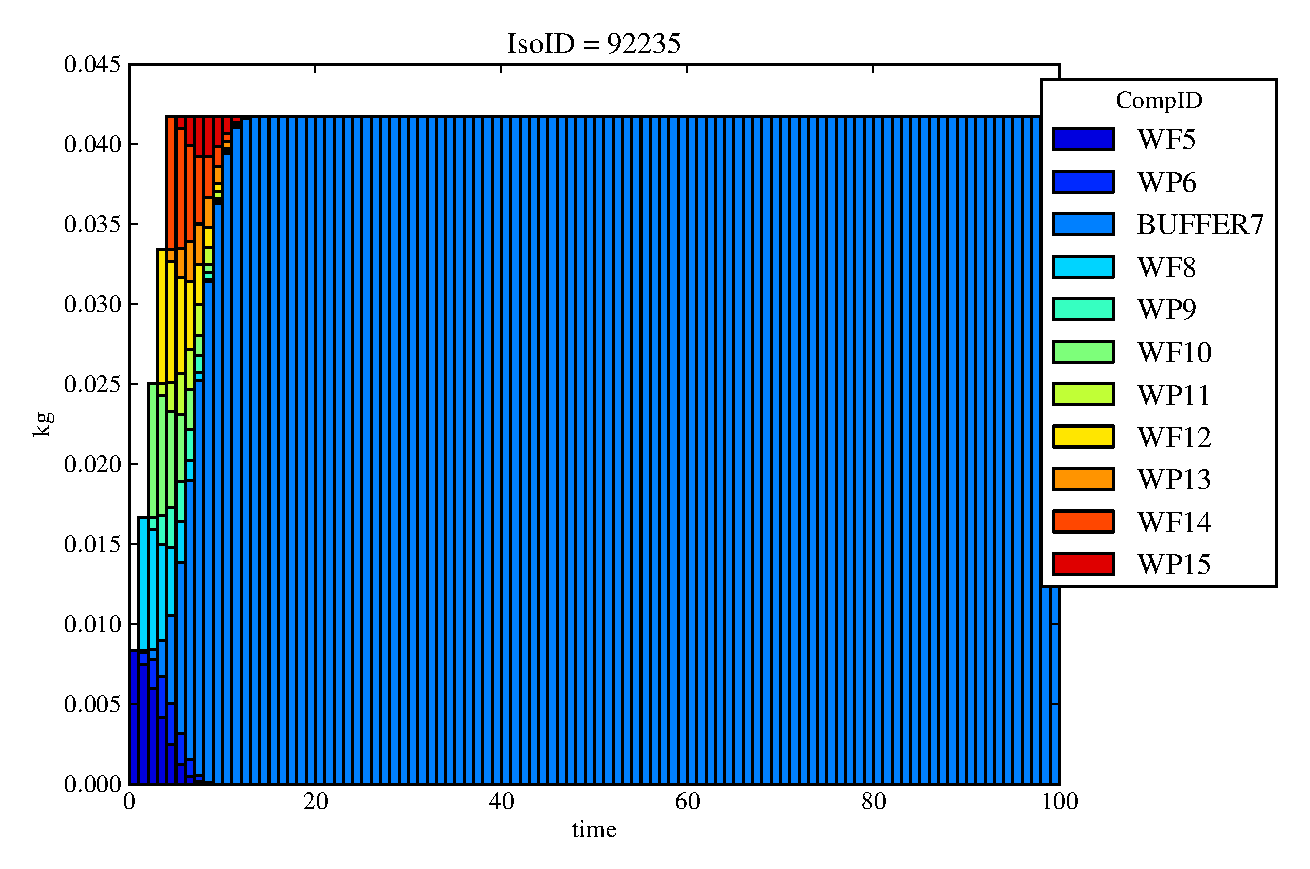
\includegraphics[width=0.6\textwidth]{./chapters/demonstration/base/drIII.eps}
\caption[$^{235}U$ residence. Degradation Rate Buffer No Release.]{
For Case DRIII, in which total containment in the buffer is assumed ($F_{d,buffer}=0$), 
$^{235}U$ travels through waste forms and waste package components ($F_d = 0.1$) before 
permanent residence in the buffer component.
}
\label{fig:drIIIall}
\begin{minipage}[b]{0.45\linewidth}

  \includegraphics[width=\textwidth]{./chapters/demonstration/base/drIII1.eps}
  \caption[Case DRIII Waste Form Contaminants.]{
    Waste Form 5 ($F_d = 0.1$) releases material with degradation. 
    }
  \label{fig:drIIIwf5}
  
  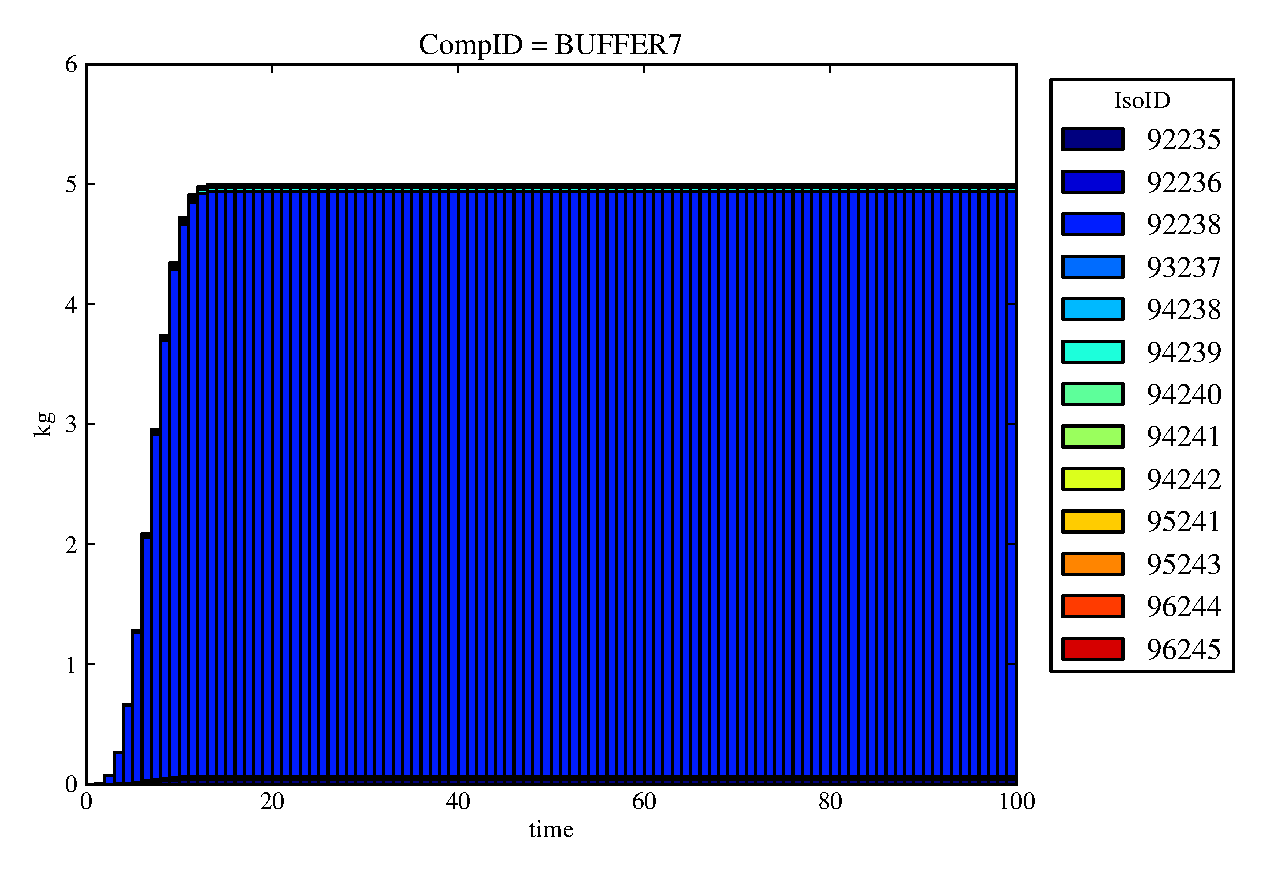
\includegraphics[width=\textwidth]{./chapters/demonstration/base/drIII3.eps}
  \caption[Case DRIII Buffer Contaminants]{
    The Buffer, component 7 ($F_d=0$), acheives total containment.
    }
  \label{fig:drIIIbuff}

\end{minipage}
\hspace{0.05\linewidth}
\begin{minipage}[b]{0.45\linewidth}
  \includegraphics[width=\textwidth]{./chapters/demonstration/base/drIII2.eps}
  \caption[Case DRIII Waste Package Contaminants.]{ 
    Waste Package 6 ($F_d = 0.1$) recieves then releases material. 
    }
  \label{fig:drIIIwp6}

  \includegraphics[width=\textwidth]{./chapters/demonstration/base/drIII0.eps}
  \caption[Case DRIII Waste Package Contaminants.]{ 
    The Far Field, component 0 ($F_d = 0.1$), never recieves material.
    }
  \label{fig:drIIIff0}


  \end{minipage}
\end{figure}
\FloatBarrier



\begin{figure}[ht]
\centering
\includegraphics[width=0.6\textwidth]{./chapters/demonstration/base/drIV.eps}
\caption[$^{235}U$ residence. Degradation Rate Buffer No Release.]{
For DRIV case in which total containment in the far field is assumed ($F_{d,ff}=0$), 
$^{235}U$ travels through interior components ($F_d = 0.1$) before 
permanent residence in the far field component.
}
\label{fig:drIVall}
\begin{minipage}[b]{0.45\linewidth}

  \includegraphics[width=\textwidth]{./chapters/demonstration/base/drIV1.eps}
  \caption[Case DRIV Waste Form Contaminants.]{
    Waste Form 5 ($F_d = 0.1$) releases material with degradation. 
    }
  \label{fig:drIVwf5}
  
  \includegraphics[width=\textwidth]{./chapters/demonstration/base/drIV3.eps}
  \caption[Case DRIV Buffer Contaminants]{
    The Buffer, component 7 ($F_d=0.0$), receives and then releases material.
    }
  \label{fig:drIVbuff}

\end{minipage}
\hspace{0.05\linewidth}
\begin{minipage}[b]{0.45\linewidth}
  \includegraphics[width=\textwidth]{./chapters/demonstration/base/drIV2.eps}
  \caption[Case DRIV Waste Package Contaminants.]{ 
    Waste Package 6 ($F_d = 0.1$) recieves then releases material. 
    }
  \label{fig:drIVwp6}

  \includegraphics[width=\textwidth]{./chapters/demonstration/base/drIV0.eps}
  \caption[Case DRIV Waste Package Contaminants.]{ 
    The Far Field, component 0 ($F_d = 0.0$), acheives total containment.
    }
  \label{fig:drIVff0}


  \end{minipage}
\end{figure}

\clearpage

\subsubsection{Mixed Cell Model}
The Mixed Cell model behaves exactly similarly to the Degradation Rate 
model, when sorption and solubility limitation in that model are disabled. When they are 
enabled, however, expected to demonstrate sorption limited and solubility 
limited transport. The extent to which sorption and solubility limitation meet 
expectations is addressed in this base case.

Dual and single parameter verification cases were run to explore the effects of sorption and 
solubility limitation both separately and together. A description of these verification 
cases can be found in Table \ref{tab:mc_base}. 
Results of these base cases can be found in Figures \ref{fig:mcI} through 
\ref{fig:mcIV}.

\begin{table}
\centering
\footnotesize{
\begin{tabularx}{\textwidth}{|X|c|c|r|r|}
  \multicolumn{5}{c}{\textbf{Mixed Cell Model No Release Contaminant Transport}}\\
  \hline
  \textbf{Case}  &  \textbf{Component} &  \textbf{Degradation Rate} & \textbf{Expected 100 yrs} & \textbf{Actual 100 yrs}\\
  \textbf{ID}    & \textbf{[Type]} &  \textbf{$[yr^{-1}]$}  &  $[\%]$  & $[\%]$\\
  \hline
  MCI     &  WF    &  0   & 100 & 100 \\ 
          &  WP    &  0.1 & 0 & 0 \\ 
          &  BUFF  &  0.1 & 0 & 0 \\ 
          &  FF    &  0.1 & 0 & 0 \\ 
  \hline
  MCII    &  WF    &  0.1 & 0 & 0 \\ 
          &  WP    &  0   & 100 & 100 \\ 
          &  BUFF  &  0.1 & 0 & 0 \\ 
          &  FF    &  0.1 & 0 & 0 \\ 
  \hline
  MCIII   &  WF    &  0.1 & 0 & 0 \\ 
          &  WP    &  0.1 & 0 & 0 \\ 
          &  BUFF  &  0   & 100 & 100 \\ 
          &  FF    &  0.1 & 0 & 0 \\ 
  \hline
  MCIV    &  WF    &  0.1 & 0 & 0 \\ 
          &  WP    &  0.1 & 0 & 0 \\ 
          &  BUFF  &  0.1 & 0 & 0 \\ 
          &  FF    &  0   & 100 & 100 \\ 
  \hline
\end{tabularx}
\caption[Mixed Cell nuclide no release results.]{Non-release behavior was 
tested for the Mixed Cell model by parameterizing each component to block 
transport.}
\label{tab:mc_base}
}
\end{table}


\begin{frame}[ctb!]
  \frametitle{Mixed Cell Model Base Case I}
\begin{figure}[ht]
\centering
\includegraphics[width=0.8\textwidth]{./images/mcI.eps}
\caption[$^{235}U$ residence. Mixed Cell Sorption Limitation Without Solubility Limitation.]{
For the MCI case in which total containment is only is assumed in the far field, 
but sorption and solubility limitation neglected, demonstrates results exactly similar to 
DRIV, as expected.}
\label{fig:mcI}
\end{figure}
\end{frame}

\begin{frame}[ctb!]
  \frametitle{Mixed Cell Model Base Case I}
  \begin{figure}[htbp!]
\begin{minipage}[b]{0.45\linewidth}

  \includegraphics[width=0.8\textwidth]{./images/mcI1.eps}
  \caption[MCI Waste Form Contaminants.]{
    Waste Form 5 ($F_d = 0.1$) releases material with degradation. 
    }
  \label{fig:mcIwf5}
  
  \includegraphics[width=0.8\textwidth]{./images/mcI3.eps}
  \caption[Case MCI Buffer Contaminants]{
    Buffer 7 ($F_d=0.1$), receives and releases material.
    }
  \label{fig:mcIbuff}

\end{minipage}
\hspace{0.05\linewidth}
\begin{minipage}[b]{0.45\linewidth}
  \includegraphics[width=0.8\textwidth]{./images/mcI2.eps}
  \caption[Case MCI Waste Package Contaminants.]{ 
    Waste Package 6 ($F_d = 0.1$) receives and releases material.
    }
  \label{fig:mcIwp6}

  \includegraphics[width=0.8\textwidth]{./images/mcI0.eps}
  \caption[Case MCI Waste Package Contaminants.]{ 
    Far Field 4 ($F_d = 0.0$) acheives full containment.
    }
  \label{fig:mcIff0}


  \end{minipage}
\end{figure}
\end{frame}

\begin{frame}[ctb!]
  \frametitle{Mixed Cell Model Base Case II}
\begin{figure}[ht]
\centering
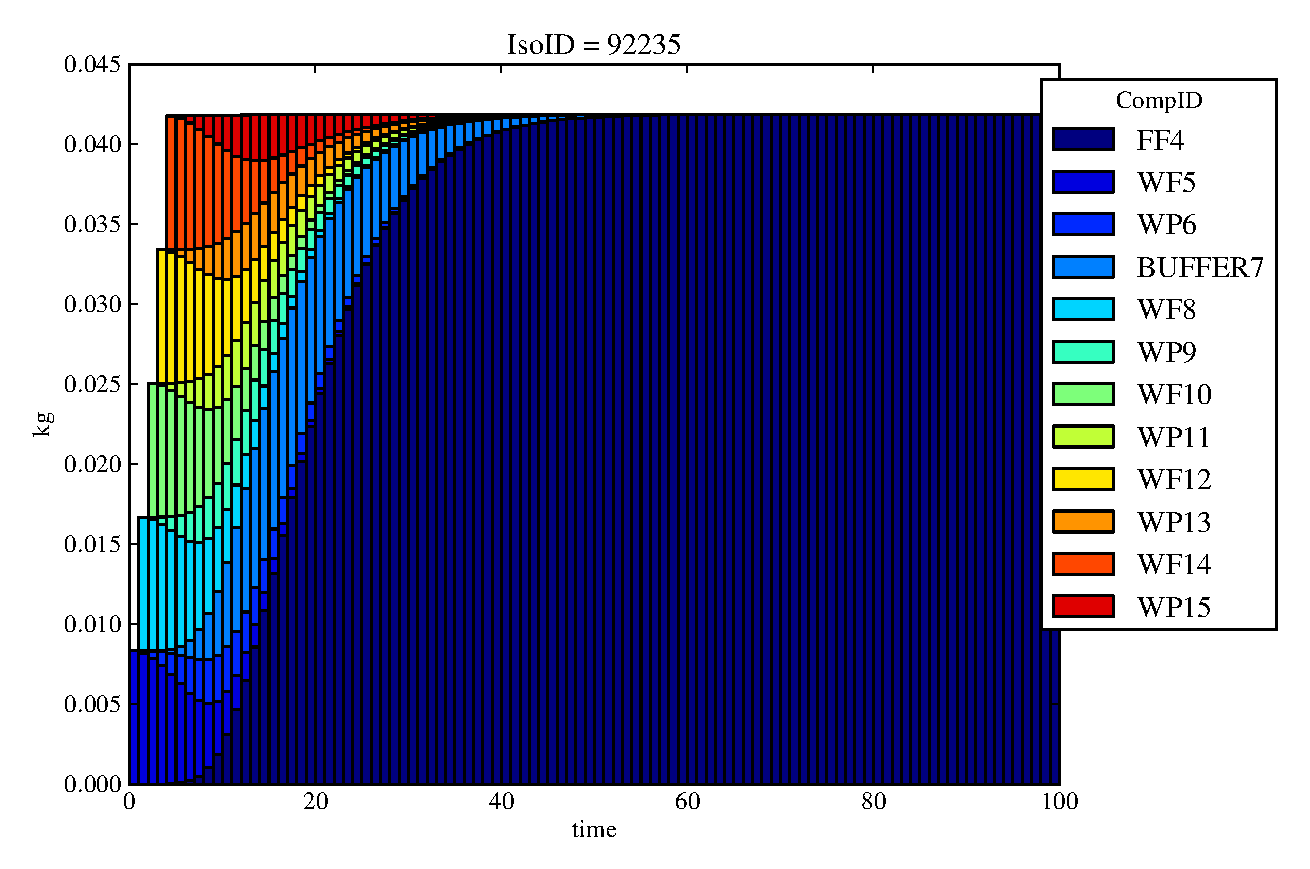
\includegraphics[width=0.8\textwidth]{./images/mcIII.eps}
\caption[$^{235}U$ residence. Mixed Cell Coupled Sorption and Solubility Limitation.]{
For the MCII case in which containment is affected by both sorption and 
solubility limitation,
($F_{d}=0.1$ for all components), $^{235}U$ travels more slowly than in the MCI case 
before permanent residence in the far field component.
}
\label{fig:mcIIIall}
\end{figure}
\end{frame}

\begin{frame}[ctb!]
  \frametitle{Mixed Cell Model Base Case II}
  \begin{figure}
\begin{minipage}[b]{0.45\linewidth}

  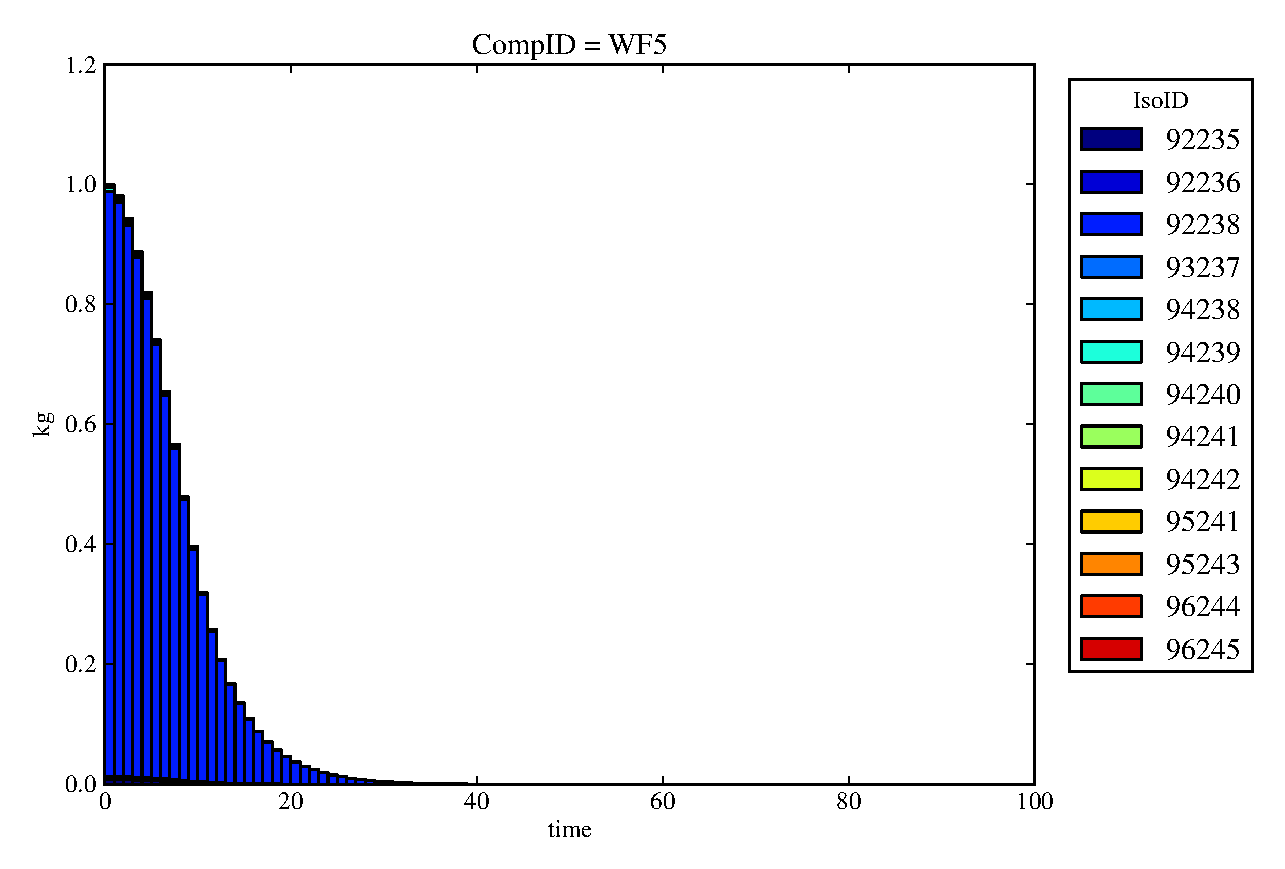
\includegraphics[width=0.8\textwidth]{./images/mcIII1.eps}
  \caption[MCI Waste Form Contaminants.]{
    Waste Form 5 ($F_d = 0.1$) releases material with degradation. 
    }
  \label{fig:mcIIIwf5}
  
  \includegraphics[width=0.8\textwidth]{./images/mcIII3.eps}
  \caption[Case MCI Buffer Contaminants]{
    Buffer 7 ($F_d=0.1$), receives and releases material.
    }
  \label{fig:mcIIIbuff}

\end{minipage}
\hspace{0.05\linewidth}
\begin{minipage}[b]{0.45\linewidth}
  \includegraphics[width=0.8\textwidth]{./images/mcIII2.eps}
  \caption[Case MCI Waste Package Contaminants.]{ 
    Waste Package 6 ($F_d = 0.1$) receives and releases material. 
    }
  \label{fig:mcIIIwp6}

  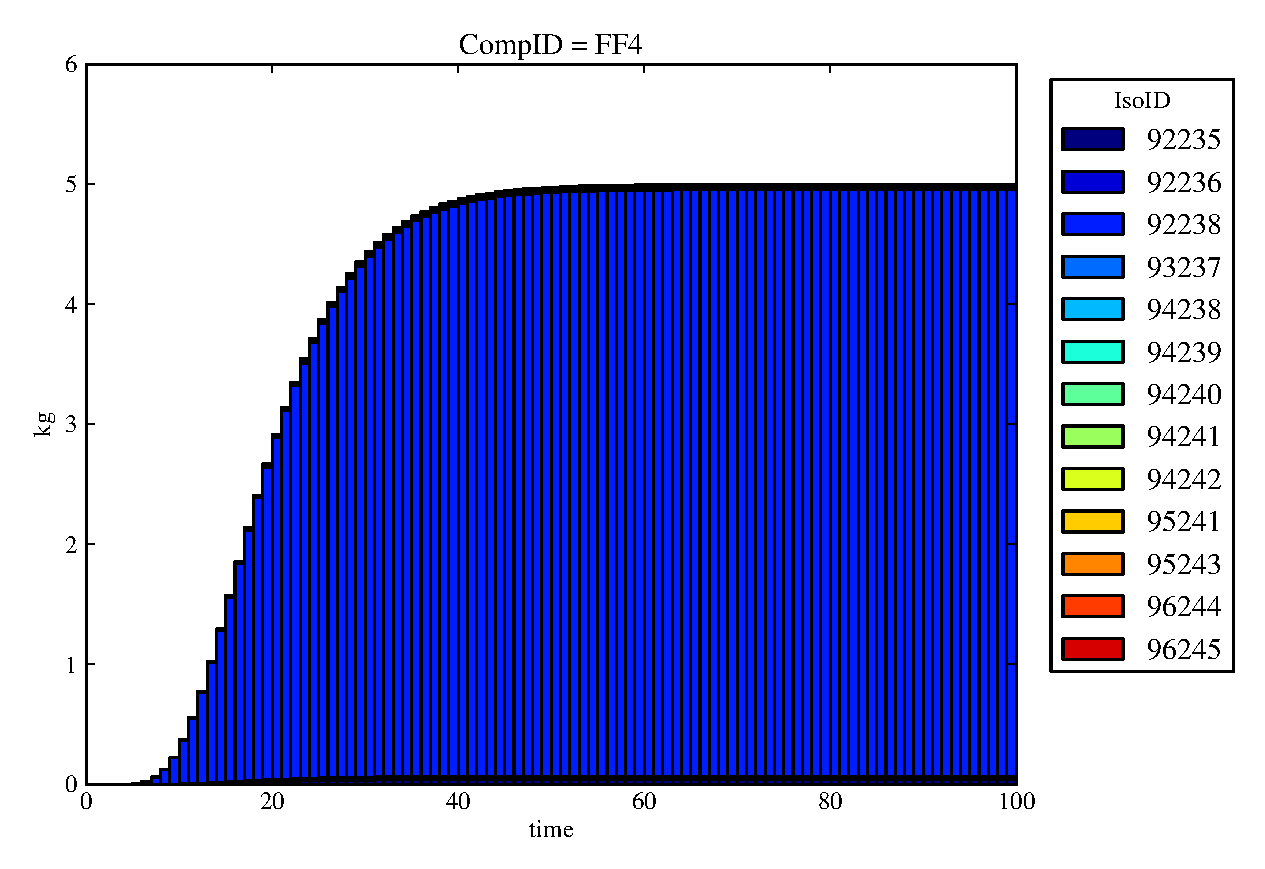
\includegraphics[width=0.8\textwidth]{./images/mcIII0.eps}
  \caption[Case MCI Waste Package Contaminants.]{ 
    Far Field 4 ($F_d = 0.1$) acheives total containment.
    }
  \label{fig:mcII}


  \end{minipage}
\end{figure}

\end{frame}

\clearpage

\subsubsection{Lumped Parameter Model}
The Lumped Parameter model, with its three formulations (Exponential Model, 
Dispersion Model, and Piston flow Model) is not expected to receive 
contaminants if the porosity or advective velocity are zero. Else, however, 
contaminants are expected to  become available to the adjacent components 
according to the functional forms of the formulations. 

To observe the behaviors of each of the three formulations and to demonstrate 
full containment in cases where it is expected, simulations were run
according to the descriptions in Table \ref{tab:lp_base}.
Results of these base cases can be found in Figures 
\ref{fig:lpEMI} through \ref{fig:lpPFMIV}.

\input{./chapters/demonstration/base/lp_base_tab}




\begin{figure}[ht]
\centering
\includegraphics[width=0.8\textwidth]{./chapters/demonstration/base/lpEMI.eps}
\caption[$^{235}U$ residence. Lumped Parameter EM Waste Form No Release.]{
For case LPEMI in which total containment in the waste form is assumed 
($F_{d,wf}=0$), $^{235}U$ 
takes permanent residence in the waste form component.
}
\label{fig:lpEMIall}
\begin{minipage}[b]{0.45\linewidth}

  \includegraphics[width=\textwidth]{./chapters/demonstration/base/lpEMI1.eps}
  \caption[LPEMI Waste Form Contaminants.]{
    Waste Form 5 ($F_d = 0.1$) releases material with degradation. 
    }
  \label{fig:lpEMIwf5}
  
  \includegraphics[width=\textwidth]{./chapters/demonstration/base/lpEMI3.eps}
  \caption[Case LPEMI Buffer Contaminants]{
    The Buffer, component 7 ($F_d=0$), acheives total containment.
    }
  \label{fig:lpEMIbuff}

\end{minipage}
\hspace{0.05\linewidth}
\begin{minipage}[b]{0.45\linewidth}
  \includegraphics[width=\textwidth]{./chapters/demonstration/base/lpEMI2.eps}
  \caption[Case LPEMI Waste Package Contaminants.]{ 
    Waste Package 6 ($F_d = 0.1$) recieves then releases material. 
    }
  \label{fig:lpEMIwp6}

  \includegraphics[width=\textwidth]{./chapters/demonstration/base/lpEMI0.eps}
  \caption[Case LPEMI Waste Package Contaminants.]{ 
    The Far Field, component 0 ($F_d = 0.1$), never recieves material.
    }
  \label{fig:lpEMIff0}


  \end{minipage}
\end{figure}
\begin{figure}[ht]
\centering
\includegraphics[width=0.8\textwidth]{./chapters/demonstration/base/lpEMII.eps}
\caption[$^{235}U$ residence. Lumped Parameter  Waste Package No Release.]{
For case LPEMII in which total containment in the waste package is assumed 
($F_{d,wp}=0$), $^{235}U$ travels through the waste form component ($F_d = 0.1$) before 
permanent residence in the waste package component.
}
\label{fig:lpEMIIall}
\begin{minipage}[b]{0.45\linewidth}

  \includegraphics[width=\textwidth]{./chapters/demonstration/base/lpEMII1.eps}
  \caption[LPEMII Waste Form Contaminants.]{
    Waste Form 5 ($F_d = 0.1$) releases material with degradation. 
    }
  \label{fig:lpEMIIwf5}
  
  \includegraphics[width=\textwidth]{./chapters/demonstration/base/lpEMII3.eps}
  \caption[Case LPEMII Buffer Contaminants]{
    The Buffer, component 7 ($F_d=0$), acheives total containment.
    }
  \label{fig:lpEMIIbuff}

\end{minipage}
\hspace{0.05\linewidth}
\begin{minipage}[b]{0.45\linewidth}
  \includegraphics[width=\textwidth]{./chapters/demonstration/base/lpEMII2.eps}
  \caption[Case LPEMII Waste Package Contaminants.]{ 
    Waste Package 6 ($F_d = 0.1$) recieves then releases material. 
    }
  \label{fig:lpEMIIwp6}

  \includegraphics[width=\textwidth]{./chapters/demonstration/base/lpEMII0.eps}
  \caption[Case LPEMII Waste Package Contaminants.]{ 
    The Far Field, component 0 ($F_d = 0.1$), never recieves material.
    }
  \label{fig:lpEMIIff0}


  \end{minipage}
\end{figure}
%\begin{figure}[ht]
%\centering
%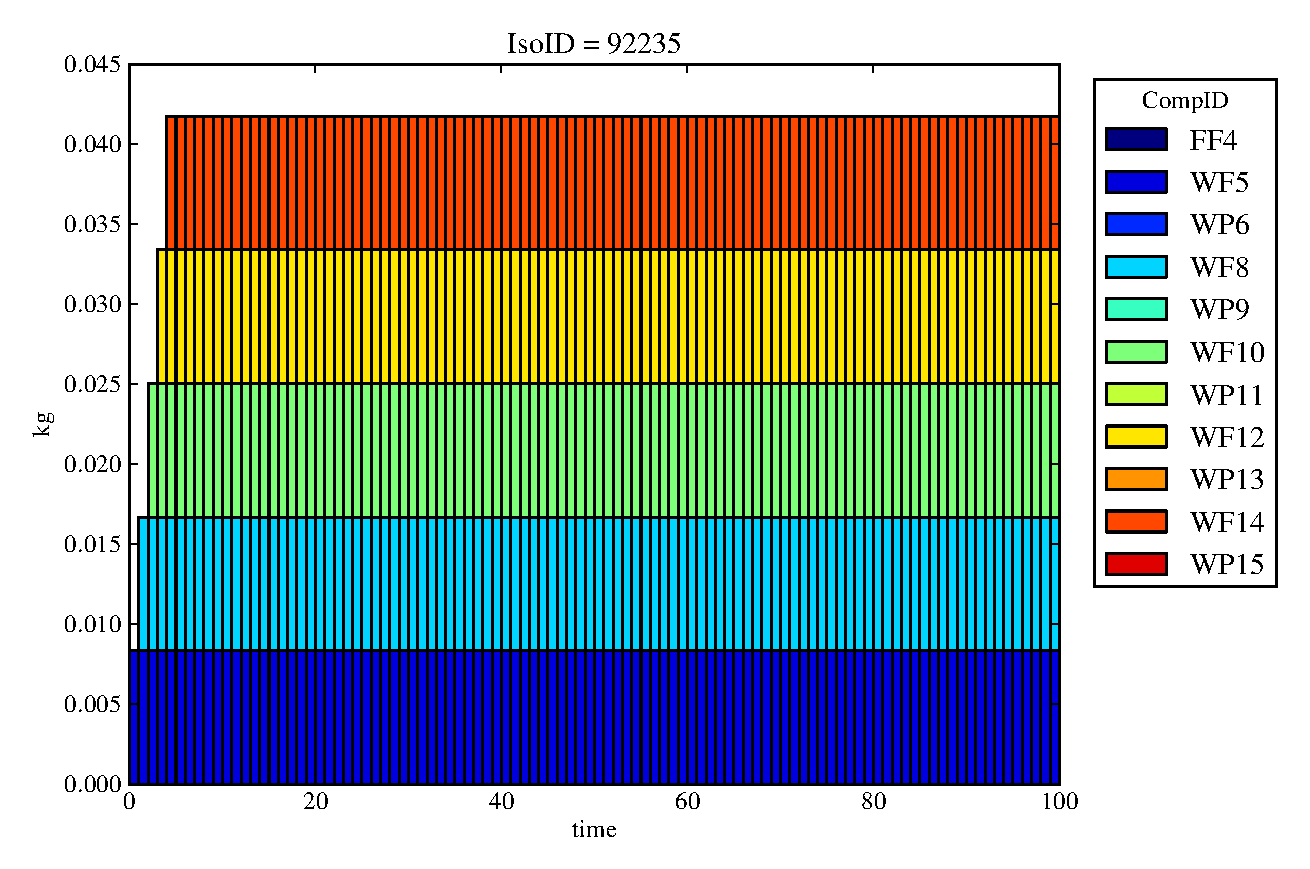
\includegraphics[width=0.8\textwidth]{./chapters/demonstration/base/lpEMIII.eps}
%\caption[$^{235}U$ residence. Lumped Parameter  <+Component+> No Release.]{
%For <+CASE+> case in which total containment in the <+component+> is assumed 
%($F_{d,<+comp+>}=0$), $^{235}U$ travels through  components ($F_d = 0.1$) before 
%permanent residence in the <+component+> component.
%}
%\label{fig:lpEMIIIall}
%\begin{minipage}[b]{0.45\linewidth}
%
%  \includegraphics[width=\textwidth]{./chapters/demonstration/base/lpEMIII1.eps}
%  \caption[LPEMIII Waste Form Contaminants.]{
%    Waste Form 5 ($F_d = 0.1$) releases material with degradation. 
%    }
%  \label{fig:lpEMIIIwf5}
%  
%  \includegraphics[width=\textwidth]{./chapters/demonstration/base/lpEMIII3.eps}
%  \caption[Case LPEMIII Buffer Contaminants]{
%    The Buffer, component 7 ($F_d=0$), acheives total containment.
%    }
%  \label{fig:lpEMIIIbuff}
%
%\end{minipage}
%\hspace{0.05\linewidth}
%\begin{minipage}[b]{0.45\linewidth}
%  \includegraphics[width=\textwidth]{./chapters/demonstration/base/lpEMIII2.eps}
%  \caption[Case LPEMIII Waste Package Contaminants.]{ 
%    Waste Package 6 ($F_d = 0.1$) recieves then releases material. 
%    }
%  \label{fig:lpEMIIIwp6}
%
%  \includegraphics[width=\textwidth]{./chapters/demonstration/base/lpEMIII0.eps}
%  \caption[Case LPEMIII Waste Package Contaminants.]{ 
%    The Far Field, component 0 ($F_d = 0.1$), never recieves material.
%    }
%  \label{fig:lpEMIIIff0}
%
%
%  \end{minipage}
%\end{figure}
%\begin{figure}[ht]
%\centering
%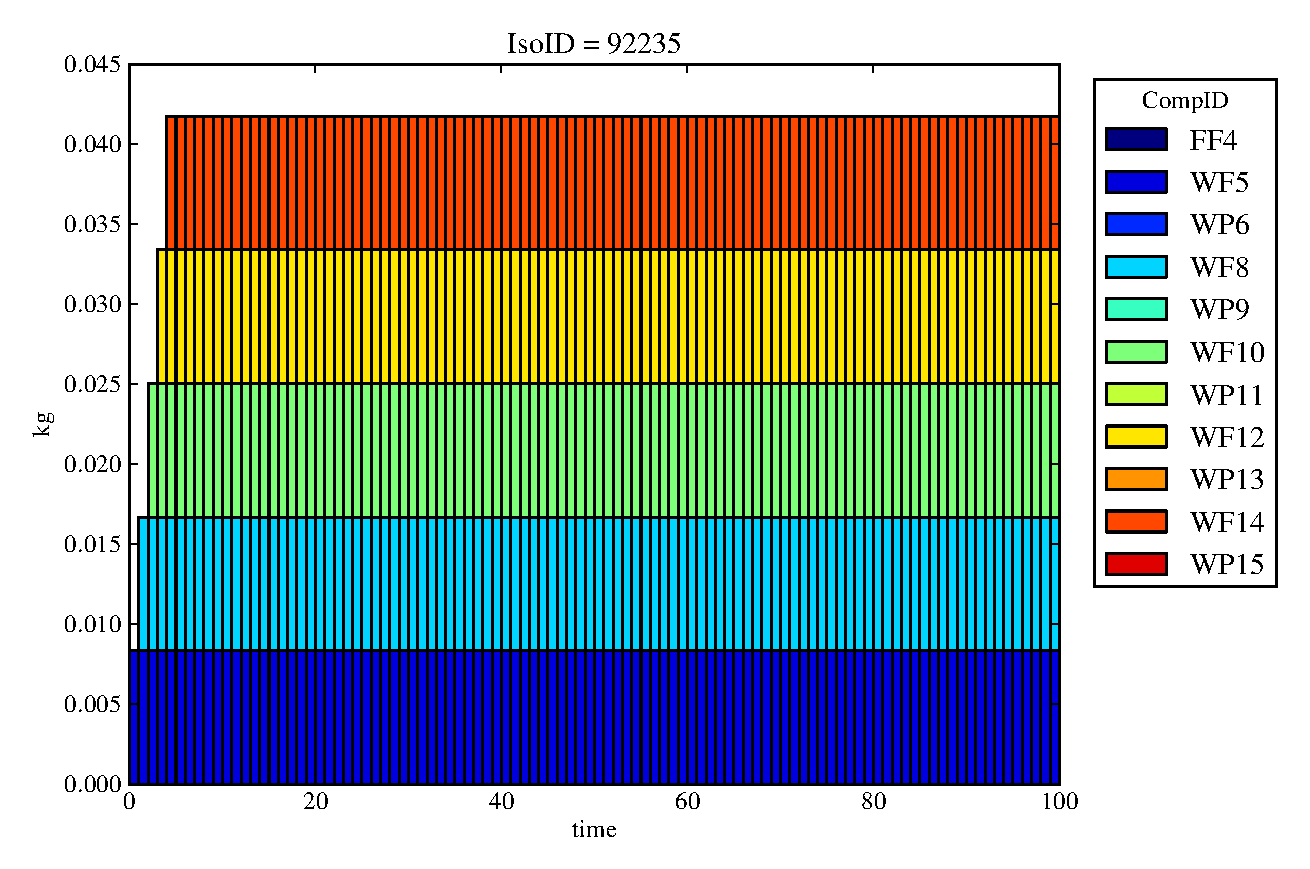
\includegraphics[width=0.8\textwidth]{./chapters/demonstration/base/lpEMIV.eps}
%\caption[$^{235}U$ residence. Lumped Parameter  <+Component+> No Release.]{
%For <+CASE+> case in which total containment in the <+component+> is assumed 
%($F_{d,<+comp+>}=0$), $^{235}U$ travels through  components ($F_d = 0.1$) before 
%permanent residence in the <+component+> component.
%}
%\label{fig:lpEMIVall}
%\begin{minipage}[b]{0.45\linewidth}
%
%  \includegraphics[width=\textwidth]{./chapters/demonstration/base/lpEMIV1.eps}
%  \caption[LPEMIV Waste Form Contaminants.]{
%    Waste Form 5 ($F_d = 0.1$) releases material with degradation. 
%    }
%  \label{fig:lpEMIVwf5}
%  
%  \includegraphics[width=\textwidth]{./chapters/demonstration/base/lpEMIV3.eps}
%  \caption[Case LPEMIV Buffer Contaminants]{
%    The Buffer, component 7 ($F_d=0$), acheives total containment.
%    }
%  \label{fig:lpEMIVbuff}
%
%\end{minipage}
%\hspace{0.05\linewidth}
%\begin{minipage}[b]{0.45\linewidth}
%  \includegraphics[width=\textwidth]{./chapters/demonstration/base/lpEMIV2.eps}
%  \caption[Case LPEMIV Waste Package Contaminants.]{ 
%    Waste Package 6 ($F_d = 0.1$) recieves then releases material. 
%    }
%  \label{fig:lpEMIVwp6}
%
%  \includegraphics[width=\textwidth]{./chapters/demonstration/base/lpEMIV0.eps}
%  caption[Case LPEMIV Waste Package Contaminants.]{ 
%    The Far Field, component 0 ($F_d = 0.1$), never recieves material.
%    }
%  \label{fig:lpEMIVff0}
%
%
%  \end{minipage}
%\end{figure}
\clearpage

%%%%%%%%%%%%%%%%%%%%%%%%%%%%%%
% DM
%%%%%%%%%%%%%%%%%%%%%%%%%%%%%%


\begin{figure}[ht]
\centering
\includegraphics[width=0.8\textwidth]{./chapters/demonstration/base/lpDMI.eps}
\caption[$^{235}U$ residence. Lumped Parameter  DM Waste Form No Release.]{
For case LPDMI  in which total containment in the waste form is assumed 
($F_{d,wf}=0$), $^{235}U$ 
takes permanent residence in the waste form  component.
}
\label{fig:lpDMIall}
\begin{minipage}[b]{0.45\linewidth}

  \includegraphics[width=\textwidth]{./chapters/demonstration/base/lpDMI1.eps}
  \caption[LPDMI Waste Form Contaminants.]{
    Waste Form 5 ($F_d = 0.1$) releases material with degradation. 
    }
  \label{fig:lpDMIwf5}
  
  \includegraphics[width=\textwidth]{./chapters/demonstration/base/lpDMI3.eps}
  \caption[Case LPDMI Buffer Contaminants]{
    The Buffer, component 7 ($F_d=0$), acheives total containment.
    }
  \label{fig:lpDMIbuff}

\end{minipage}
\hspace{0.05\linewidth}
\begin{minipage}[b]{0.45\linewidth}
  \includegraphics[width=\textwidth]{./chapters/demonstration/base/lpDMI2.eps}
  \caption[Case LPDMI Waste Package Contaminants.]{ 
    Waste Package 6 ($F_d = 0.1$) recieves then releases material. 
    }
  \label{fig:lpDMIwp6}

  \includegraphics[width=\textwidth]{./chapters/demonstration/base/lpDMI0.eps}
  \caption[Case LPDMI Waste Package Contaminants.]{ 
    The Far Field, component 0 ($F_d = 0.1$), never recieves material.
    }
  \label{fig:lpDMIff0}


  \end{minipage}
\end{figure}
\begin{figure}[ht]
\centering
\includegraphics[width=0.8\textwidth]{./chapters/demonstration/base/lpDMII.eps}
\caption[$^{235}U$ residence. Lumped Parameter  DM Waste Package No Release.]{
For LPDMII case in which total containment in the waste package is assumed 
($F_{d,wp}=0$), $^{235}U$ travels through the waste form component ($F_d = 0.1$) before 
permanent residence in the waste form component.
}
\label{fig:lpDMIIall}
\begin{minipage}[b]{0.45\linewidth}

  \includegraphics[width=\textwidth]{./chapters/demonstration/base/lpDMII1.eps}
  \caption[LPDMII Waste Form Contaminants.]{
    Waste Form 5 ($F_d = 0.1$) releases material with degradation. 
    }
  \label{fig:lpDMIIwf5}
  
  \includegraphics[width=\textwidth]{./chapters/demonstration/base/lpDMII3.eps}
  \caption[Case LPDMII Buffer Contaminants]{
    The Buffer, component 7 ($F_d=0$), acheives total containment.
    }
  \label{fig:lpDMIIbuff}

\end{minipage}
\hspace{0.05\linewidth}
\begin{minipage}[b]{0.45\linewidth}
  \includegraphics[width=\textwidth]{./chapters/demonstration/base/lpDMII2.eps}
  \caption[Case LPDMII Waste Package Contaminants.]{ 
    Waste Package 6 ($F_d = 0.1$) recieves then releases material. 
    }
  \label{fig:lpDMIIwp6}

  \includegraphics[width=\textwidth]{./chapters/demonstration/base/lpDMII0.eps}
  \caption[Case LPDMII Waste Package Contaminants.]{ 
    The Far Field, component 0 ($F_d = 0.1$), never recieves material.
    }
  \label{fig:lpDMIIff0}


  \end{minipage}
\end{figure}
%\begin{figure}[ht]
%\centering
%\includegraphics[width=0.8\textwidth]{./chapters/demonstration/base/lpDMIII.eps}
%\caption[$^{235}U$ residence. Lumped Parameter  <+Component+> No Release.]{
%For <+CASE+> case in which total containment in the <+component+> is assumed 
%($F_{d,<+comp+>}=0$), $^{235}U$ travels through  components ($F_d = 0.1$) before 
%permanent residence in the <+component+> component.
%}
%\label{fig:lpDMIIIall}
%\begin{minipage}[b]{0.45\linewidth}
%
%  \includegraphics[width=\textwidth]{./chapters/demonstration/base/lpDMIII1.eps}
%  \caption[LPDMIII Waste Form Contaminants.]{
%    Waste Form 5 ($F_d = 0.1$) releases material with degradation. 
%    }
%  \label{fig:lpDMIIIwf5}
%  
%  \includegraphics[width=\textwidth]{./chapters/demonstration/base/lpDMIII3.eps}
%  \caption[Case LPDMIII Buffer Contaminants]{
%    The Buffer, component 7 ($F_d=0$), acheives total containment.
%    }
%  \label{fig:lpDMIIIbuff}
%
%\end{minipage}
%\hspace{0.05\linewidth}
%\begin{minipage}[b]{0.45\linewidth}
%  \includegraphics[width=\textwidth]{./chapters/demonstration/base/lpDMIII2.eps}
%  \caption[Case LPDMIII Waste Package Contaminants.]{ 
%    Waste Package 6 ($F_d = 0.1$) recieves then releases material. 
%    }
%  \label{fig:lpDMIIIwp6}
%
%  \includegraphics[width=\textwidth]{./chapters/demonstration/base/lpDMIII0.eps}
%  \caption[Case LPDMIII Waste Package Contaminants.]{ 
%    The Far Field, component 0 ($F_d = 0.1$), never recieves material.
%    }
%  \label{fig:lpDMIIIff0}
%
%
%  \end{minipage}
%\end{figure}
%\begin{figure}[ht]
%\centering
%\includegraphics[width=0.8\textwidth]{./chapters/demonstration/base/lpDMIV.eps}
%\caption[$^{235}U$ residence. Lumped Parameter  <+Component+> No Release.]{
%For <+CASE+> case in which total containment in the <+component+> is assumed 
%($F_{d,<+comp+>}=0$), $^{235}U$ travels through  components ($F_d = 0.1$) before 
%permanent residence in the <+component+> component.
%}
%\label{fig:lpDMIVall}
%\begin{minipage}[b]{0.45\linewidth}
%
%  \includegraphics[width=\textwidth]{./chapters/demonstration/base/lpDMIV1.eps}
%  \caption[LPDMIV Waste Form Contaminants.]{
%    Waste Form 5 ($F_d = 0.1$) releases material with degradation. 
%    }
%  \label{fig:lpDMIVwf5}
%  
%  \includegraphics[width=\textwidth]{./chapters/demonstration/base/lpDMIV3.eps}
%  \caption[Case LPDMIV Buffer Contaminants]{
%    The Buffer, component 7 ($F_d=0$), acheives total containment.
%    }
%  \label{fig:lpDMIVbuff}
%
%\end{minipage}
%\hspace{0.05\linewidth}
%\begin{minipage}[b]{0.45\linewidth}
%  \includegraphics[width=\textwidth]{./chapters/demonstration/base/lpDMIV2.eps}
%  \caption[Case LPDMIV Waste Package Contaminants.]{ 
%    Waste Package 6 ($F_d = 0.1$) recieves then releases material. 
%    }
%  \label{fig:lpDMIVwp6}
%
%  \includegraphics[width=\textwidth]{./chapters/demonstration/base/lpDMIV0.eps}
%  caption[Case LPDMIV Waste Package Contaminants.]{ 
%    The Far Field, component 0 ($F_d = 0.1$), never recieves material.
%    }
%  \label{fig:lpDMIVff0}
%
%
%  \end{minipage}
%\end{figure}
\clearpage
%%%%%%%%%%%%%%%%%%%%%%%%%%%%%%%
% PFM
%%%%%%%%%%%%%%%%%%%%%%%%%%%%%%%



\begin{figure}[ht]
\centering
\includegraphics[width=0.8\textwidth]{./chapters/demonstration/base/lpPFMI.eps}
\caption[$^{235}U$ residence. Lumped Parameter PFM Waste Form No Release.]{
For case LPPFMI  in which total containment in the waste form is assumed 
($F_{d,wf}=0$), $^{235}U$ resides permanently in the waste form component.
}
\label{fig:lpPFMIall}
\begin{minipage}[b]{0.45\linewidth}

  \includegraphics[width=\textwidth]{./chapters/demonstration/base/lpPFMI1.eps}
  \caption[LPPFMI Waste Form Contaminants.]{
    Waste Form 5 ($F_d = 0.1$) releases material with degradation. 
    }
  \label{fig:lpPFMIwf5}
  
  \includegraphics[width=\textwidth]{./chapters/demonstration/base/lpPFMI3.eps}
  \caption[Case LPPFMI Buffer Contaminants]{
    The Buffer, component 7 ($F_d=0$), acheives total containment.
    }
  \label{fig:lpPFMIbuff}

\end{minipage}
\hspace{0.05\linewidth}
\begin{minipage}[b]{0.45\linewidth}
  \includegraphics[width=\textwidth]{./chapters/demonstration/base/lpPFMI2.eps}
  \caption[Case LPPFMI Waste Package Contaminants.]{ 
    Waste Package 6 ($F_d = 0.1$) recieves then releases material. 
    }
  \label{fig:lpPFMIwp6}

  \includegraphics[width=\textwidth]{./chapters/demonstration/base/lpPFMI0.eps}
  \caption[Case LPPFMI Waste Package Contaminants.]{ 
    The Far Field, component 0 ($F_d = 0.1$), never recieves material.
    }
  \label{fig:lpPFMIff0}


  \end{minipage}
\end{figure}
\begin{figure}[ht]
\centering
\includegraphics[width=0.8\textwidth]{./chapters/demonstration/base/lpPFMII.eps}
\caption[$^{235}U$ residence. Lumped Parameter PFM Waste Package No Release.]{
For case LPPFMII in which total containment in the waste package is assumed 
($F_{d,wp}=0$), $^{235}U$ travels through the waste form component ($F_d = 0.1$) before 
permanent residence in the waste package component.
}
\label{fig:lpPFMIIall}
\begin{minipage}[b]{0.45\linewidth}

  \includegraphics[width=\textwidth]{./chapters/demonstration/base/lpPFMII1.eps}
  \caption[LPPFMII Waste Form Contaminants.]{
    Waste Form 5 ($F_d = 0.1$) releases material with degradation. 
    }
  \label{fig:lpPFMIIwf5}
  
  \includegraphics[width=\textwidth]{./chapters/demonstration/base/lpPFMII3.eps}
  \caption[Case LPPFMII Buffer Contaminants]{
    The Buffer, component 7 ($F_d=0$), acheives total containment.
    }
  \label{fig:lpPFMIIbuff}

\end{minipage}
\hspace{0.05\linewidth}
\begin{minipage}[b]{0.45\linewidth}
  \includegraphics[width=\textwidth]{./chapters/demonstration/base/lpPFMII2.eps}
  \caption[Case LPPFMII Waste Package Contaminants.]{ 
    Waste Package 6 ($F_d = 0.1$) recieves then releases material. 
    }
  \label{fig:lpPFMIIwp6}

  \includegraphics[width=\textwidth]{./chapters/demonstration/base/lpPFMII0.eps}
  \caption[Case LPPFMII Waste Package Contaminants.]{ 
    The Far Field, component 0 ($F_d = 0.1$), never recieves material.
    }
  \label{fig:lpPFMIIff0}


  \end{minipage}
\end{figure}
%\begin{figure}[ht]
%\centering
%\includegraphics[width=0.8\textwidth]{./chapters/demonstration/base/lpPFMIII.eps}
%\caption[$^{235}U$ residence. Lumped Parameter  <+Component+> No Release.]{
%For <+CASE+> case in which total containment in the <+component+> is assumed 
%($F_{d,<+comp+>}=0$), $^{235}U$ travels through  components ($F_d = 0.1$) before 
%permanent residence in the <+component+> component.
%}
%\label{fig:lpPFMIIIall}
%\begin{minipage}[b]{0.45\linewidth}
%
%  \includegraphics[width=\textwidth]{./chapters/demonstration/base/lpPFMIII1.eps}
%  \caption[LPPFMIII Waste Form Contaminants.]{
%    Waste Form 5 ($F_d = 0.1$) releases material with degradation. 
%    }
%  \label{fig:lpPFMIIIwf5}
%  
%  \includegraphics[width=\textwidth]{./chapters/demonstration/base/lpPFMIII3.eps}
%  \caption[Case LPPFMIII Buffer Contaminants]{
%    The Buffer, component 7 ($F_d=0$), acheives total containment.
%    }
%  \label{fig:lpPFMIIIbuff}
%
%\end{minipage}
%\hspace{0.05\linewidth}
%\begin{minipage}[b]{0.45\linewidth}
%  \includegraphics[width=\textwidth]{./chapters/demonstration/base/lpPFMIII2.eps}
%  \caption[Case LPPFMIII Waste Package Contaminants.]{ 
%    Waste Package 6 ($F_d = 0.1$) recieves then releases material. 
%    }
%  \label{fig:lpPFMIIIwp6}
%
%  \includegraphics[width=\textwidth]{./chapters/demonstration/base/lpPFMIII0.eps}
%  \caption[Case LPPFMIII Waste Package Contaminants.]{ 
%    The Far Field, component 0 ($F_d = 0.1$), never recieves material.
%    }
%  \label{fig:lpPFMIIIff0}
%
%
%  \end{minipage}
%\end{figure}
%\begin{figure}[ht]
%\centering
%\includegraphics[width=0.8\textwidth]{./chapters/demonstration/base/lpPFMIV.eps}
%\caption[$^{235}U$ residence. Lumped Parameter  <+Component+> No Release.]{
%For <+CASE+> case in which total containment in the <+component+> is assumed 
%($F_{d,<+comp+>}=0$), $^{235}U$ travels through  components ($F_d = 0.1$) before 
%permanent residence in the <+component+> component.
%}
%\label{fig:lpPFMIVall}
%\begin{minipage}[b]{0.45\linewidth}
%
%  \includegraphics[width=\textwidth]{./chapters/demonstration/base/lpPFMIV1.eps}
%  \caption[LPPFMIV Waste Form Contaminants.]{
%    Waste Form 5 ($F_d = 0.1$) releases material with degradation. 
%    }
%  \label{fig:lpPFMIVwf5}
%  
%  \includegraphics[width=\textwidth]{./chapters/demonstration/base/lpPFMIV3.eps}
%  \caption[Case LPPFMIV Buffer Contaminants]{
%    The Buffer, component 7 ($F_d=0$), acheives total containment.
%    }
%  \label{fig:lpPFMIVbuff}
%
%\end{minipage}
%\hspace{0.05\linewidth}
%\begin{minipage}[b]{0.45\linewidth}
%  \includegraphics[width=\textwidth]{./chapters/demonstration/base/lpPFMIV2.eps}
%  \caption[Case LPPFMIV Waste Package Contaminants.]{ 
%    Waste Package 6 ($F_d = 0.1$) recieves then releases material. 
%    }
%  \label{fig:lpPFMIVwp6}
%
%  \includegraphics[width=\textwidth]{./chapters/demonstration/base/lpPFMIV0.eps}
%  caption[Case LPPFMIV Waste Package Contaminants.]{ 
%    The Far Field, component 0 ($F_d = 0.1$), never recieves material.
%    }
%  \label{fig:lpPFMIVff0}
%
%
%  \end{minipage}
%\end{figure}

\clearpage

\subsubsection{One Dimensional Advective Dispersive Model}
The One Dimensional Advective Dispersive Model contaminants if the porosity is 
zero or if both the reference diffusivity and advective velocity are zero. 
Else, however, contaminants are expected to  become available to the adjacent 
components according to the analytical form of the solution.

To observe the behavior of the solution and to demonstrate full containment in 
cases where it is expected, simulations were run according to the descriptions 
in Table \ref{tab:1d_base}.  Results of these base cases can be found in 
Figures \ref{fig:1dI} through \ref{fig:1dIV}.  

\input{./chapters/demonstration/base/1d_base_tab}

\begin{figure}[ht]
\centering
\includegraphics[width=0.8\textwidth]{./chapters/demonstration/base/od.eps}
\caption[1 Dimensional PPM Model.]{
For the case in which transport through all components is represented by the 1 
Dimensional PPM model, material moves very slowly into the far field. Indeed, 
so slowly that the time steps are measured in 10s of years.
}
\label{fig:1dppmall}
\begin{minipage}[b]{0.45\linewidth}

  \includegraphics[width=\textwidth]{./chapters/demonstration/base/od2.eps}
  \caption[Case ODI Waste Form Contaminants.]{
    Waste Form 5 releases material at a slow, nearly constant rate into Waste 
    Package 6.
    }
  \label{fig:drIVwf5}
  \includegraphics[width=\textwidth]{./chapters/demonstration/base/od3.eps}
  \caption[Case ODI Buffer Contaminants]{
    The Buffer, component 7 very slowly receives material at a slow, nearly 
    constant rate. It then very slowly releases material.
    }
  \label{fig:drIVbuff}
\end{minipage}
\hspace{0.05\linewidth}
\begin{minipage}[b]{0.45\linewidth}
  \includegraphics[width=\textwidth]{./chapters/demonstration/base/od1.eps}
  \caption[Case ODI Waste Package Contaminants.]{ 
    Waste Package 6 very slowly recieves then very slowly releases material. 
    }
  \label{fig:drIVwp6}
  \includegraphics[width=\textwidth]{./chapters/demonstration/base/od0.eps}
  \caption[Case ODI Waste Package Contaminants.]{ 
    The Far Field, component 4, acheives total containment.
    }
  \label{fig:drIVff0}


  \end{minipage}
\end{figure}

\clearpage
